\documentclass{ltxdoc}
\usepackage[T1]{fontenc}
\usepackage{lmodern}
\usepackage{morefloats}
\usepackage[svgnames]{xcolor}
\usepackage{tikz}
\usetikzlibrary{tqft}
\usepackage[numbered]{hypdoc}
\definecolor{lstbgcolor}{rgb}{0.9,0.9,0.9} 
 
\usepackage{listings}
\lstloadlanguages{[LaTeX]TeX}
\lstset{breakatwhitespace=true,breaklines=true,language=TeX}
 
\usepackage{fancyvrb}

\newenvironment{example}
  {\VerbatimEnvironment
   \begin{VerbatimOut}{example.out}}
  {\end{VerbatimOut}
   \begin{center}
   \setlength{\parindent}{0pt}
   \fbox{\begin{minipage}{.9\linewidth}
     \lstset{breakatwhitespace=true,breaklines=true,language=TeX,basicstyle=\small}
     \lstinputlisting[]{example.out}
   \end{minipage}}

   \fbox{\begin{minipage}{.9\linewidth}
     \centering
     \input{example.out}
   \end{minipage}}
\end{center}
}

\providecommand*{\url}{\texttt}

\title{The \textsf{tqft} TikZ Library: Documentation}
\author{Andrew Stacey \\ \url{stacey@math.ntnu.no}}

\begin{document}

\maketitle

\begin{center}
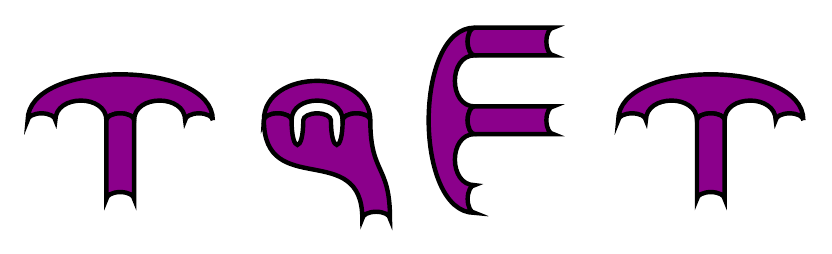
\begin{tikzpicture}[
    scale=.5,
    every tqft/.style={
      transform shape
    },
    tqft/cobordism/.style={
      fill=DarkMagenta,
      draw,
      ultra thick},
  ]
  \pic[
    name=a,
    tqft,
    incoming boundary components=0,
    outgoing boundary components=3,
  ];
  \pic[
    name=b,
    at=(a-outgoing boundary 2),
    tqft cylinder,
    anchor=incoming boundary 1,
  ];
  \pic[
    at=(a-outgoing boundary 3),
    name=c,
    tqft,
    incoming boundary components=0,
    outgoing boundary components=2,
    anchor={(0,1)},
  ];
  \pic[
    at=(c-outgoing boundary 1),
    name=d,
    tqft,
    incoming boundary components=3,
    outgoing boundary components=1,
    offset=2.5,
    anchor=incoming boundary 1,
    boundary separation=1cm,
    cobordism height=2.5cm,
  ];
  \pic[
    at=(c-outgoing boundary 2),
    name=e,
    tqft,
    rotate=90,
    incoming boundary components=0,
    outgoing boundary components=3,
    anchor={(2,-.5)}
  ];
  \pic[
    at=(e-outgoing boundary 3),
    name=f,
    tqft cylinder,
    rotate=90,
    anchor=incoming boundary 1,
  ];
  \pic[
    at=(e-outgoing boundary 2),
    name=g,
    tqft cylinder,
    rotate=90,
    anchor=incoming boundary 1,
  ];
  \pic[
    at=(g-outgoing boundary 1),
    name=h,
    tqft,
    anchor={(0,1)},
    incoming boundary components=0,
    outgoing boundary components=3,
  ];
  \pic[
    at=(h-outgoing boundary 2),
    name=i,
    tqft cylinder,
    anchor=incoming boundary 1,
  ];
\end{tikzpicture}
\end{center}

\section{Introduction}
This package defines some TikZ/PGF node shapes that can be used to construct the diagrams common in Topological Quantum Field Theory (TQFT).
An example follows:

\begin{example}
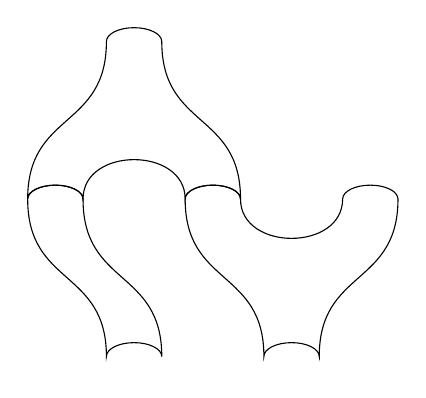
\begin{tikzpicture}[tqft/cobordism/.style={draw}]
\pic[tqft/pair of pants,name=a];
\pic[tqft/cylinder to next,anchor=incoming boundary 1,name=c,at=(a-outgoing boundary 1)];
\pic[tqft/reverse pair of pants, anchor=incoming boundary 1,at=(a-outgoing boundary 2)];
\end{tikzpicture}
\end{example}

Before giving any details, a word is in order about the keys involved in this package.
There are many options and keys that can be set via the \Verb+\pgfkeys+ system (which is used for setting options in Ti\emph{k}Z).
Such keys live in a ``directory'' but often that can be omitted.
For example, in the Ti\emph{k}Z command \Verb+\draw[red] (0,0) -- (1,0);+ the key \Verb+red+ is actually in the ``directory'' \Verb+/tikz+ but it is not necessary to specify that as it is assumed.
Defining a ``directory'' helps separate keys and ensure that there is no conflict.
The keys in this library are (mostly) defined in the directory \Verb+/tikz/tqft+ but the very first call to a \Verb+tqft+ key will (in general) set the ``current directory'' to \Verb+/tikz/tqft+ and so all subsequent keys do not need prefixing.
Moreover, any unknown keys are passed on to the \Verb+/tikz+ directory so there is (or should be!) no harm in mixing \Verb+tqft+ specific keys with ordinary Ti\emph{k}Z keys.
Some examples take advantage of this switch so when copying and modifying examples from this document, it is important to remember that the first \Verb+tqft+ specific key needs an explicit \Verb+tqft/+ prefix.
More detailed information is in the section on styling.

\section{The Shapes}

There is only one picture shape: \Verb+cobordism+.
This is a cobordism between a number of incoming circles and a number of outgoing circles, where the numbers of boundary components can be specified as options to the shape.
There are certain common shapes that are predefined as aliases to the main shape with specified boundaries.
The list of predefined shapes follows.
The names are all in the \Verb+tqft+ family, but an alias is made so that \Verb+tqft shape+ will work without any further qualification.

\begin{enumerate}
\item \Verb+pair of pants+

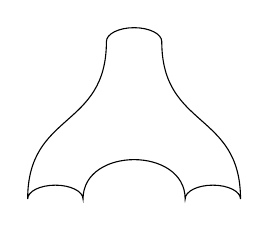
\begin{tikzpicture}
\pic[draw,tqft/pair of pants];
\end{tikzpicture}

\item \Verb+reverse pair of pants+

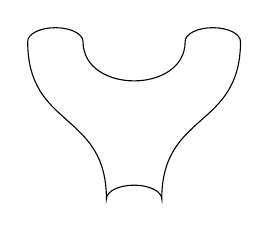
\begin{tikzpicture}
\pic[draw,tqft/reverse pair of pants];
\end{tikzpicture}

\item \Verb+cylinder to prior+

This is a cylinder that has been skewed to one side, thus following the same path as the \Verb+pair of pants+ cobordism but with only one outgoing boundary component.
The name \Verb+to prior+ is because it goes towards the lower-numbered component on the \Verb+pair of pants+. 

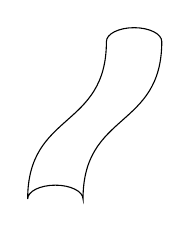
\begin{tikzpicture}
\pic[draw,tqft/cylinder to prior];
\end{tikzpicture}

\item \Verb+cylinder to next+

This is a cylinder that has been skewed to one side, thus following the same path as the \Verb+pair of pants+ cobordism but with only one outgoing boundary component.
The name \Verb+to next+ is because it goes towards the higher-numbered component on the \Verb+pair of pants+. 

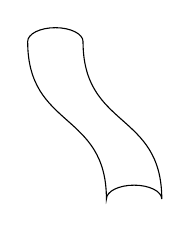
\begin{tikzpicture}
\pic[draw,tqft/cylinder to next];
\end{tikzpicture}

\item \Verb+cylinder+

This is a straight cylinder.

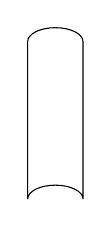
\begin{tikzpicture}
\pic[draw,tqft/cylinder];
\end{tikzpicture}

\item \Verb+cap+

This is a cap.

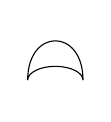
\begin{tikzpicture}
\pic[draw,tqft/cap];
\end{tikzpicture}

\item \Verb+cup+

This is a cup (an upside-down cap).

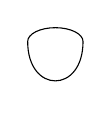
\begin{tikzpicture}
\pic[draw,tqft/cup];
\end{tikzpicture}

\end{enumerate}

The general shape is controlled by the following keys:

\begin{itemize}
\item \DescribeMacro{view from} To get a simulated 3D effect, the cobordism is drawn as if viewed from a slight angle.
The value of this key determines whether the cobordism is viewed from the direction of the incoming boundary components or the outgoing ones.
This key can take the values \Verb+incoming+ and \Verb+outgoing+.
The default is \Verb+outgoing+.
\item \DescribeMacro{cobordism height} This is the height of the cobordism (``height'' interpreted in its own internal coordinate system).
With no offset (q.v.), this would be the distance between the centres of the first incoming and first outgoing boundary components.

\item \DescribeMacro{boundary separation} This is the distance between the centres of the boundary components of the same type.

\item \DescribeMacro{circle x radius} This is the half-width of the boundary circles.

\item \DescribeMacro{circle y radius} This is the half-depth of the boundary circles (``depth'' since, in the internal coordinate system, this corresponds to the \(z\)-axis out of the page).

\item \DescribeMacro{incoming boundary components} The number of incoming boundary components (can be zero).

\item \DescribeMacro{outgoing boundary components} The number of outgoing boundary components (can be zero).

\item \DescribeMacro{offset} This offsets the first outgoing boundary component horizontally relative to the first incoming boundary component.
It is a dimensionless number (not necessarily an integer) and is interpreted so that a value of \(1\) aligns the first outgoing boundary component with the second incoming boundary component.

\item \DescribeMacro{genus} This defines the number of holes in the shape.
These are spread out in a horizontal line in the middle of the shape.
\end{itemize}

\section{Styling}

There are various options for styling the diagrams.
To understand how they work, it is important to know the order in which a cobordism is drawn and how many pieces it decomposes into.
This is the following list, with the corresponding key:

\begin{enumerate}
\item The boundary circles are drawn.
These are actually elliptical nodes.
Applicable styles:

\begin{itemize}
\item \Verb+every boundary component+,
\item \Verb+every incoming boundary component+, or  \Verb+every outgoing boundary component+,
\item \Verb+incoming boundary component <n>+, or \Verb+outgoing boundary component <n>+
\end{itemize}

\item The lower edges of the boundary circles are redrawn.
These are arcs.

\begin{itemize}
\item \Verb+every lower boundary component+,
\item \Verb+every incoming lower boundary component+, or  \Verb+every outgoing lower boundary component+,
\item \Verb+incoming lower boundary component <n>+, or \Verb+outgoing lower boundary component <n>+
\end{itemize}

\item The full edge of the cobordism is drawn.
This is a closed path so can be sensibly filled.
It is clipped against a path defined by the genus of the cobordism which results in holes if it is filled (or shaded or anything else that goes in to the interior).

\begin{itemize}
\item \Verb+cobordism+,
\item also, any actions specified on the \Verb+pic+ are applied here (see the \Verb+pic actions+ key in the TikZ manual for full details on this).
\end{itemize}

\item Any holes specified by the genus are now drawn.
These are styled to give the 3D impression, and this follows the direction specified by the \Verb+view from+ key.

\begin{itemize}
\item \Verb+cobordism+, this style is applied because the curves defined by the genus can be thought of as part of the edge of the cobordism shape.
However, following this key then \Verb+fill=none+ is issued.
This is because even if the main shape is filled, the paths drawing the holes should almost certainly not be.
\item \Verb+cobordism edge+, the same logic applies to the edge path (q.v.).
\item \Verb+genus style+.
\end{itemize}

\item The non-boundary edge of the cobordism is redrawn.

\begin{itemize}
\item \Verb+cobordism edge+,
\item \Verb+cobordism outer edge+
\end{itemize}

\item The upper edges of the boundary circles are redrawn.

\begin{itemize}
\item \Verb+every upper boundary component+,
\item \Verb+every incoming upper boundary component+, or  \Verb+every outgoing upper boundary component+,
\item \Verb+incoming upper boundary component <n>+, or \Verb+outgoing upper boundary component <n>+
\end{itemize}
\end{enumerate}

The fact that there are so many is to allow different style to be applied to different pieces and to give as much control as possible, whilst still making it fairly straightforward to draw a simple cobordism.
The duplication of paths is to allow certain composite pieces to be \emph{filled}.
Here is a progressively built up cobordism.

\begin{example}
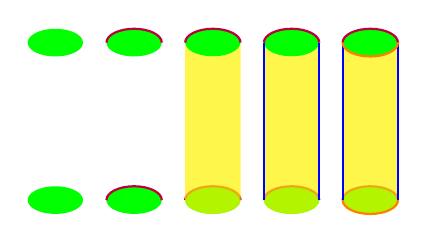
\begin{tikzpicture}[tqft/view from=incoming]
\begin{scope}[tqft/every boundary component/.style={fill=green,fill opacity=1}]
\pic[tqft/cylinder,at={(1,0)}];
\begin{scope}[tqft/every lower boundary component/.style={draw=purple,thick}]
\pic[tqft/cylinder,at={(2,0)}];
\begin{scope}[tqft/cobordism/.style={fill=yellow,fill opacity=.7}]
\pic[tqft/cylinder,at={(3,0)}];
\begin{scope}[tqft/cobordism edge/.style={draw,thick,blue}]
\pic[tqft/cylinder,fill=yellow,fill opacity=.7,at={(4,0)}];
\begin{scope}[tqft/every upper boundary component/.style={draw,thick,orange}]
\pic[tqft/cylinder,fill=yellow,fill opacity=.7,at={(5,0)}];
\end{scope}
\end{scope}
\end{scope}
\end{scope}
\end{scope}
\end{tikzpicture}
\end{example}

\section{Anchors}

The cobordism is a \Verb+pic+ so does not have any native anchors.
Nevertheless, a multitude of coordinates are defined that simulate the anchors associated with nodes.
There is also support for specifying the shape to be located relative to a particular anchor.

The \Verb+\pic+ should be named via the \Verb+name=<prefix>+ key, whereupon the anchors are prefixed by this value.
The pseudo-anchors defined have the naming convention \Verb+<prefix>-<anchor name>+.
They are:
%
\begin{itemize}
\item \Verb+incoming boundary <n>+, these are in fact elliptical nodes and so also define actual anchors.
\item \Verb+incoming boundary+ is an alias for \Verb+incoming boundary 1+.
\item \Verb+outgoing boundary <n>+, same.
\item \Verb+outgoing boundary+ is an alias for \Verb+outgoing boundary 1+.
\item \Verb=between incoming <n> and <n+1>=, this lies on the midpoint of the curve between successive boundary components.
\item \Verb=between outgoing <n> and <n+1>=, this lies on the midpoint of the curve between successive boundary components.
\item \Verb=between first incoming and first outgoing= is on the edge between the first incoming and first outgoing boundary components; note that this is only defined if there are both incoming and outgoing boundary components.
\item \Verb=between last incoming and last outgoing= is on the edge between the last incoming and last outgoing boundary components; note that this is only defined if there are both incoming and outgoing boundary components.
\item \Verb=between first and last incoming=; this is only defined if there are no outgoing components.
\item \Verb=between first and last outgoing=; this is only defined if there are no incoming components.
\item \Verb=hole <n>=; if the genus is non-zero, this points to the centre of the \(n\)th hole.
\end{itemize}

To place the shape relative to an anchor, use the \Verb+anchor+ key.
The argument should be just the name of the anchor without the \Verb+<prefix>-+.
The \Verb+anchor+ key can also take another type of argument.
If its argument is of the form \Verb+(x,y)+ then this is taken as a pseudo-coordinate.
It is interpreted as being \(x\) boundary components across and \(y\) times the cobordism height down.
However, if an \Verb+offset+ is specified then the resulting \(x\) value is shifted so that if \(y < 0\) then \((1,y)\) is in line with the first incoming boundary component and if \(y > 1\) then \((1,y)\) is in line with the first outgoing boundary component.
If \(0 < y < 1\) then \((1,y)\) linearly interpolates between the first incoming and first outgoing boundary components.
Thus \((1,0)\) is the first incoming boundary component, \((1,1)\) the first outgoing boundary component, \((0,0)\) is one unit to the left of the first incoming, and \((1,2)\) one unit below the first outgoing.
Note that the picture is shifted to put this point at the current coordinate.

\begin{example}
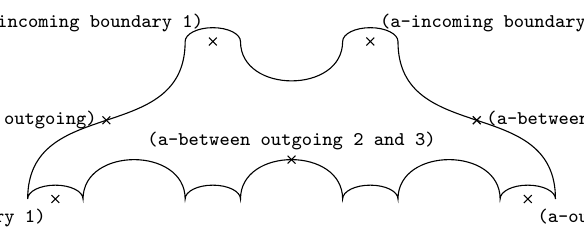
\begin{tikzpicture}
\pic[tqft, incoming boundary components=2,outgoing boundary components=4,offset=-1,draw,name=a];
\foreach \anchor/\placement in
{
between first incoming and first outgoing/left,
between last incoming and last outgoing/right,
between outgoing 2 and 3/above,
incoming boundary 1/above left,
incoming boundary 2/above right,
outgoing boundary 1/below left,
outgoing boundary 4/below right}
\draw[overlay,shift=(a-\anchor)] plot[mark=x] coordinates{(0,0)} node[\placement] {\scriptsize\texttt{(a-\anchor)}};
\end{tikzpicture}
\end{example}

\section{Notes}

\begin{enumerate}
\item Like \Verb+node+s, \Verb+pic+s need the \Verb+transform shape+ key to be set to take note of external transformations (other than shifts).
\item There is an additional \Verb+every tqft+ key which is run when the \Verb+tqft+ key is invoked (which might be via some other key).
This is better placed than the \Verb+every pic+ key since that applies to a surrounding scope rather than to the \Verb+pic+ itself.
\item If the \Verb+tqft+ key is invoked, either implicitly or explicitly, then the \Verb+pic type+ is set to \Verb+cobordism+.
This has the side effect that the invoking syntax has to be completely set by keys; so the \Verb+pic (<name>) at (<coord>) {<type>}+ cannot be used.
Rather, the \Verb+name+ and \Verb+at+ have to be specified by keys and the \Verb+type+ omitted.
\end{enumerate}

\section{More Examples}

\begin{example}
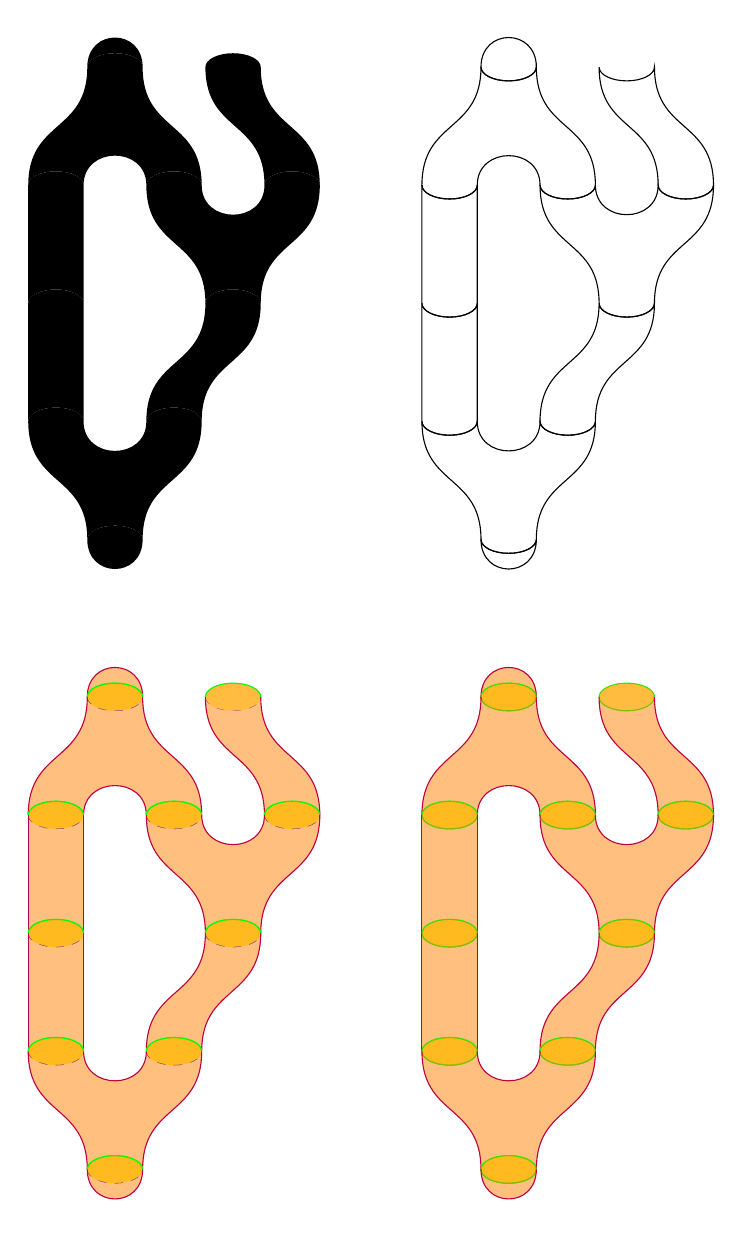
\begin{tikzpicture}[tqft/cobordism height=1.5cm,tqft/boundary  separation=1.5cm]
\foreach \coord/\style in {
{(0,0)}/{tqft/view from=outgoing,fill},
{(5,0)}/{tqft/view from=incoming,draw},
{(0,-8)}/{fill=orange,fill opacity=.5,tqft/every lower boundary component/.style={draw,blue,ultra thin,dashed},tqft/every upper boundary component/.style={draw,green},tqft/cobordism edge/.style={draw,purple},tqft/every boundary component/.style={fill=yellow}},
{(5,-8)}/{fill=orange,fill opacity=.5,tqft/cobordism edge/.style={draw,purple},tqft/every boundary component/.style={fill=yellow,draw=green}}
} {
\begin{scope}
\edef\styleit{\noexpand\tikzset{every tqft/.style={\style}}}
\styleit
\pic[tqft/cap,name=h,at=\coord];
\pic[tqft/pair of pants,anchor=incoming boundary 1,name=a,at=(h-outgoing boundary 1)];
\pic[tqft/cylinder to next,anchor={(0,1)},name=d,at=(a-outgoing boundary 2)];
\pic[tqft/reverse pair of pants,anchor=incoming boundary 1,name=b,at=(a-outgoing boundary 2)];
\pic[tqft/cylinder to prior,anchor=incoming boundary 1,name=c,at=(b-outgoing boundary 1)];
\pic[tqft/cylinder,anchor=incoming boundary 1,name=e,at=(a-outgoing  boundary 1)];
\pic[tqft/cylinder,anchor=incoming boundary 1,name=f,at=(e-outgoing  boundary 1)];
\pic[tqft/reverse pair of pants,anchor=incoming boundary 1,name=g,at=(f-outgoing boundary 1)];
\pic[tqft/cup,anchor=incoming boundary 1,name=i,at=(g-outgoing boundary 1)];
\end{scope}
}
\end{tikzpicture}
\end{example}

\begin{example}
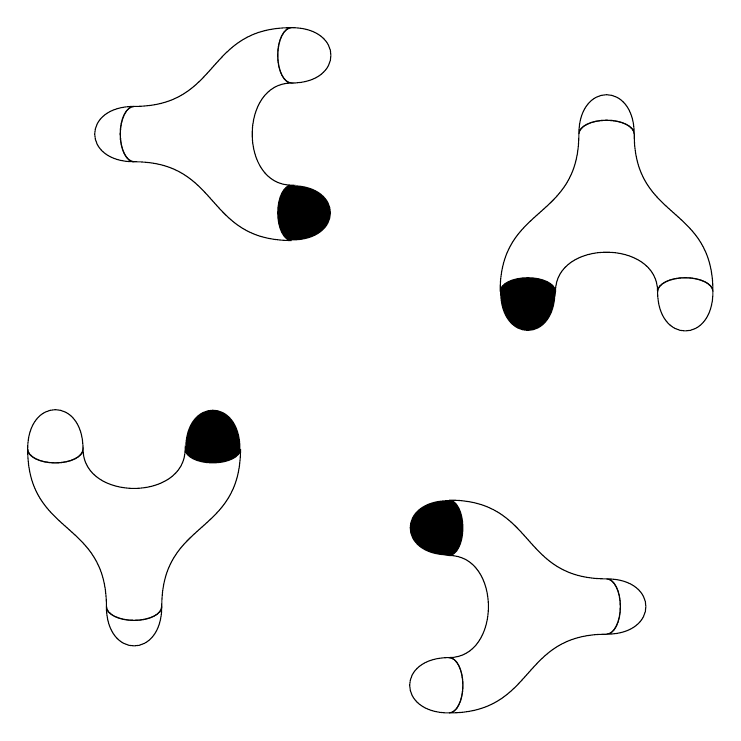
\begin{tikzpicture}[every tqft/.append style={transform shape}]
\foreach \ang in {0,90,180,270} {
\begin{scope}[rotate=\ang]
\pic[draw,tqft/pair of pants,name=a,at={(3,3)}];
\pic[draw,tqft/cap,anchor=outgoing boundary 1,at=(a-incoming boundary 1)];
\pic[fill,tqft/cup,anchor=incoming boundary 1,at=(a-outgoing boundary 1)];
\pic[draw,tqft/cup,anchor=incoming boundary 1,at=(a-outgoing boundary 2)];
\end{scope}
}
\end{tikzpicture}
\end{example}
\end{document}